\chapter{Design and architecture}

\section{User interface}

\begin{figure}[H]
  \centering
    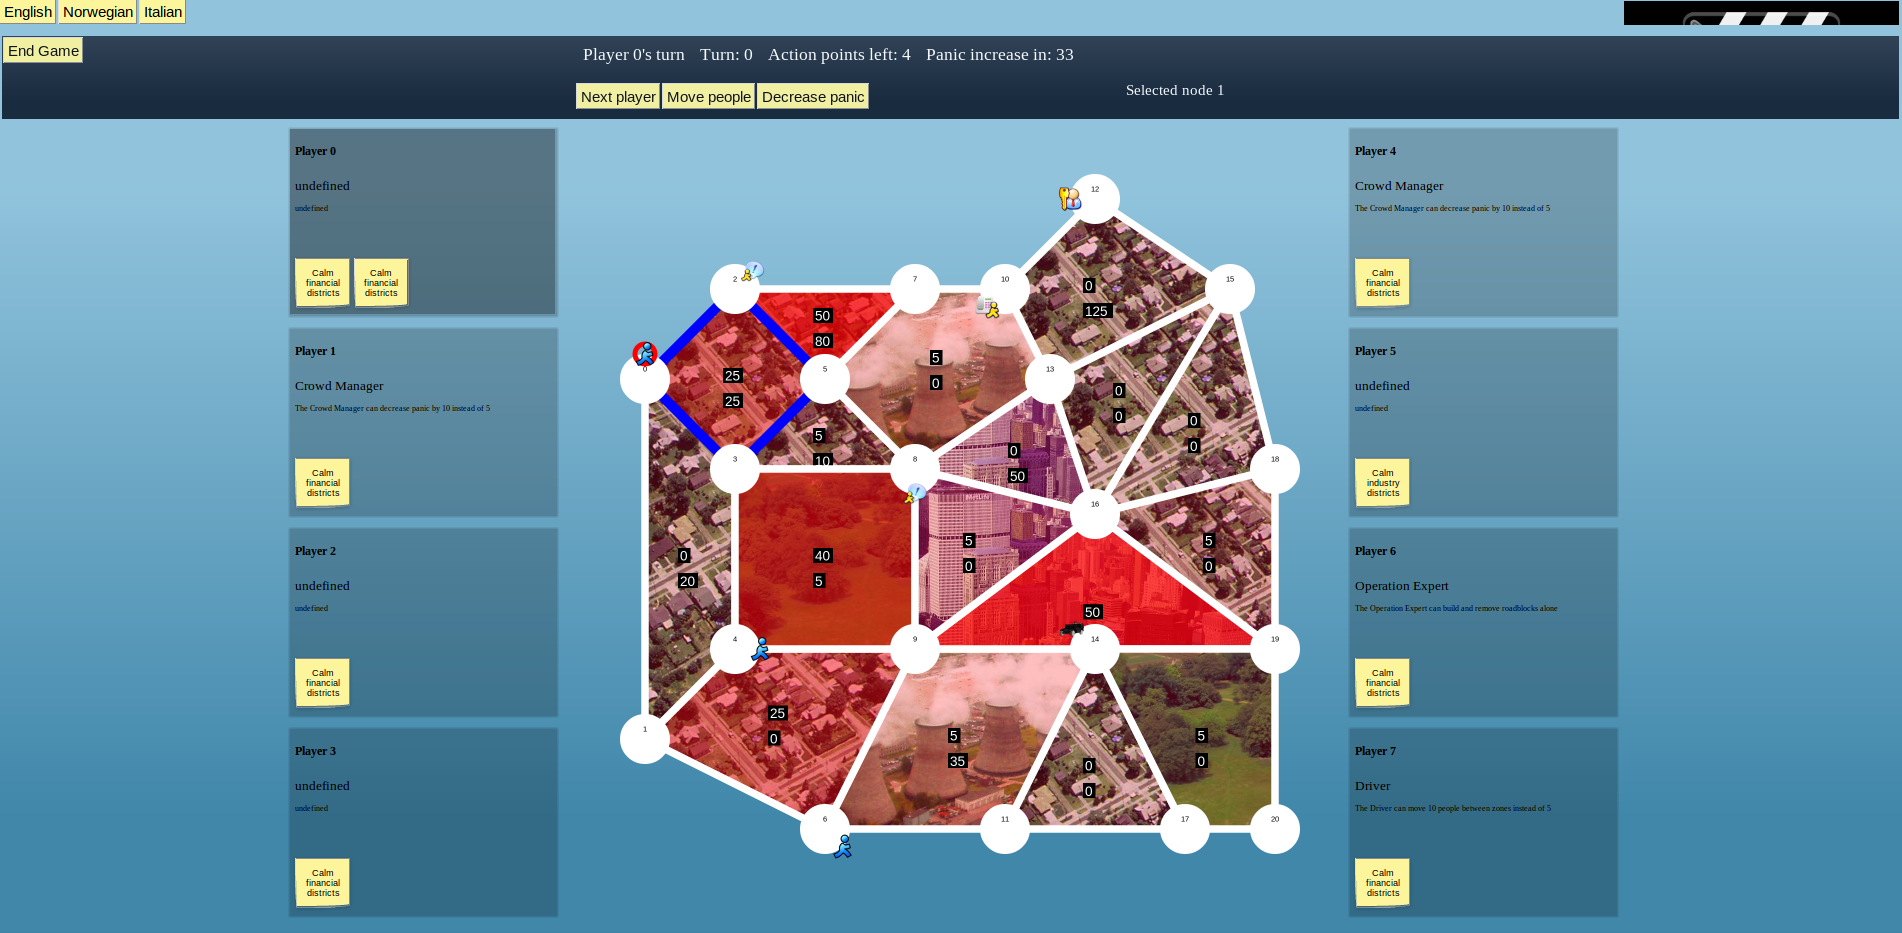
\includegraphics[width=1.0\textwidth]{img/gamefinal.png}
  \caption{User interface, ' The user interface of the game, complete with a board, pieces, cards and information tables'} 
  \label{fig:finalgamegui}
\end{figure}









\subsection{User interface design}

The customer had already designed a physical board game of Don’t Panic, which formed the basis for designing the electronic version. In the earliest stages of the designing Balsamiq Mockups was used, an online tool for interface designing.\\
\\
Mockups is designed to be an easy and efficient tool used in the early stages of interface designing, and it can be used to generate click-through prototypes for interfaces. Through myBalsamiq it can also be used as a collaborative tool, supporting project-based collaboration and real-time changes.\\






\subsection{Realisation of the user interface}

The main part of the interface is the HTML5 canvas. The board and pieces of the game are all drawn within this canvas using JavaScript. The players are able to control their respective player pieces by dragging them on the board from one node to another using the mouse, like one would do using the hands when playing the physical version of the board game. One of the main goals of the project was to preserve the physical interaction of playing a board game in the electronic version, so it was decided that implementing a drag-and-drop functionality for the player pieces would be a good idea. \\
\\
The panic levels for each zone are printed inside the zones. This was very cumbersome with the physical version, as the players were forced to update all the zones manually each time the timer counted down, as well as when event cards and information affected the zones. This is now handled automatically on the server. \\


\begin{figure}[H]
  \centering
    
\includegraphics[width=1.0\textwidth]{img/statusbar.png}
  \caption{User interface, 'Status bar'} 
  \label{fig:statusbar}
\end{figure}

An information table is placed above the canvas. This table contains the button the players would use when ending their turns, as well as buttons for placing information centers and roadblocks on the nodes they are located. The table also contains information about whose turn it is, how many turns have passed, how many actions the active player has left and a timer which counts down to the next increase in panic. \\
\\
On each side of the canvas there are sidebar rows. Players have their own row, which is highlighted when it is their turn. The rows contain information on players, as well as their information cards. Since this is a collaborative game, all the cards should be visible to the players so they can openly discuss how the cards should be used, as well as trade cards between themselves. This preserves the verbal interaction dynamics of a physical board game. The cards are implemented as buttons with text corresponding to their effect in the game. \\

\begin{figure}[H]
  \centering
    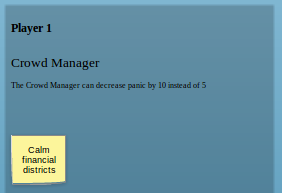
\includegraphics[width=0.4\textwidth]{img/playerinfo.png}
  \caption{User interface, 'Player Information'} 
  \label{fig:playerinfo}
\end{figure}




\section{Client/Server architecture}
A client-server model was chosen as the architectural pattern. This was highly desired by the customer, as they wanted different clients
to work with the server. Therefore using a different architecture was never considered as an option.

\subsection{Initial suggestion for a high level architecture from the customer}

\begin{figure}[H]
  \centering
    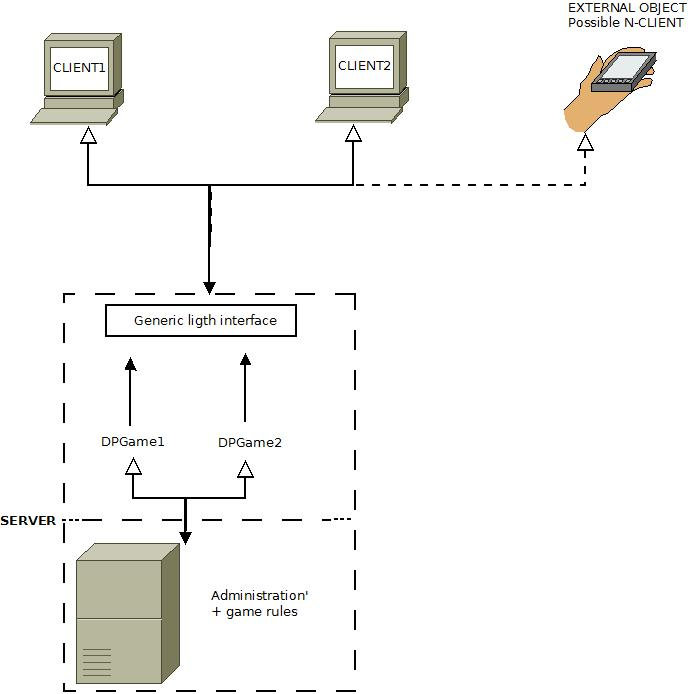
\includegraphics[width=1.0\textwidth]{img/Client-serverarchitecture.jpeg}
  \caption{System architecture, 'Initial suggestion from customer'} 
  \label{fig:initialsuggestion}
\end{figure}



\subsection{High level system architecture}

\begin{figure}[H]
  \centering
    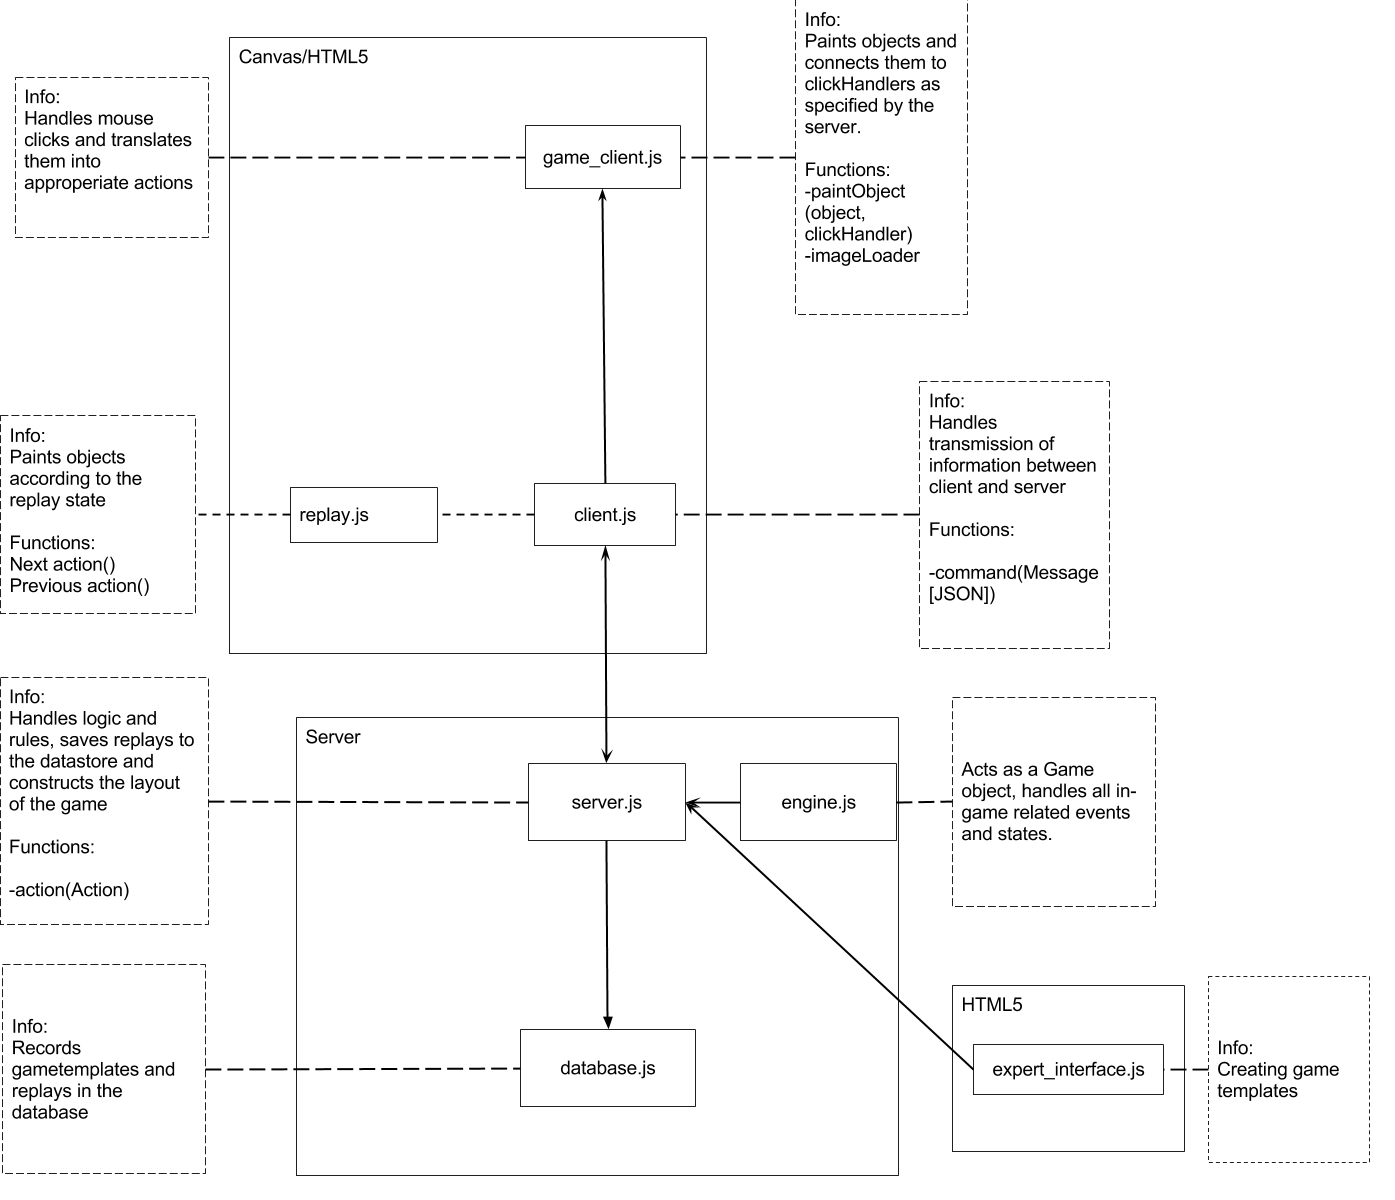
\includegraphics[width=1.0\textwidth]{img/highlevelarch.png}
  \caption{System architecture, 'High level system architecture'} 
  \label{fig:highsysarch}
\end{figure}

\subsection{Object diagram}

\begin{figure}[H]
  \centering
    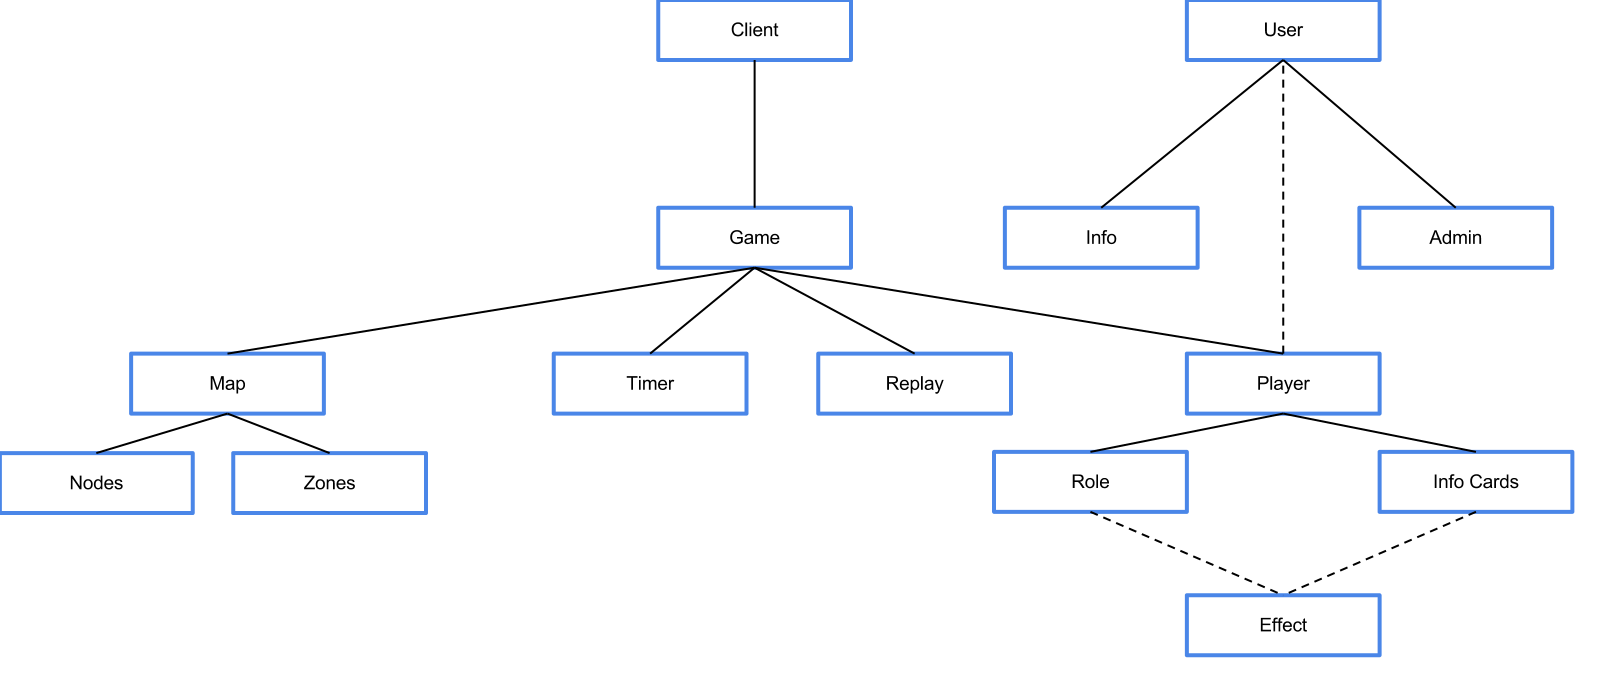
\includegraphics[width=1.0\textwidth]{img/GameTree.png}
  \caption{Object diagram, 'Game tree'} 
  \label{fig:gametree}
\end{figure}


\subsection{ER diagram}
\begin{figure}[H]
  \centering
    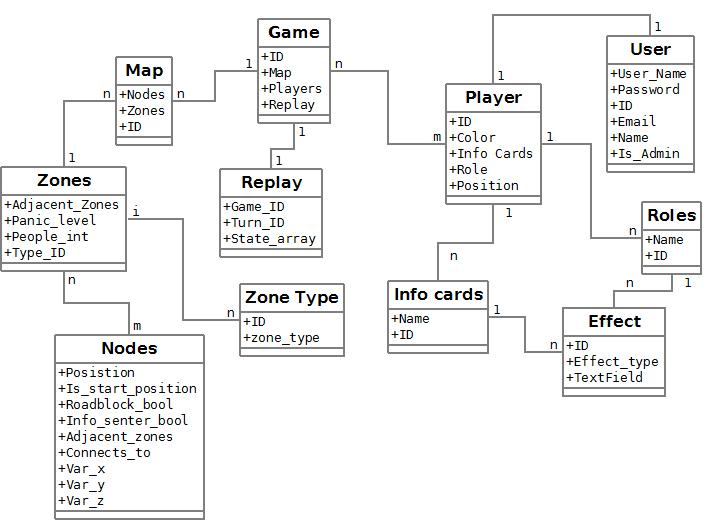
\includegraphics[width=1.0\textwidth]{img/erdiagram.jpeg}
  \caption{'ER diagram'} 
  \label{fig:erdiagram}
\end{figure}

\subsection{Final ER diagram}
\begin{figure}[H]
  \centering
    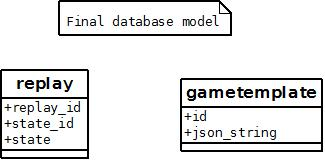
\includegraphics[width=1.0\textwidth]{img/finaldatabase.jpeg}
  \caption{'Final ER diagram'} 
  \label{fig:final_erdiagram}
\end{figure}

\subsection{Object hierarchy}
This chart is intended to show a high level view of the hierarchy, and how the objects are connected together to avoid loops. 

\subsection{Sequence diagrams}

The sequence diagrams show the interactions between the files, functions and methods. It depicts the objects and files interactions in the right time sequence. The diagrams also show the calls each method or a file sends to the next file, function or method.  \\


\begin{figure}[H]
  \centering
    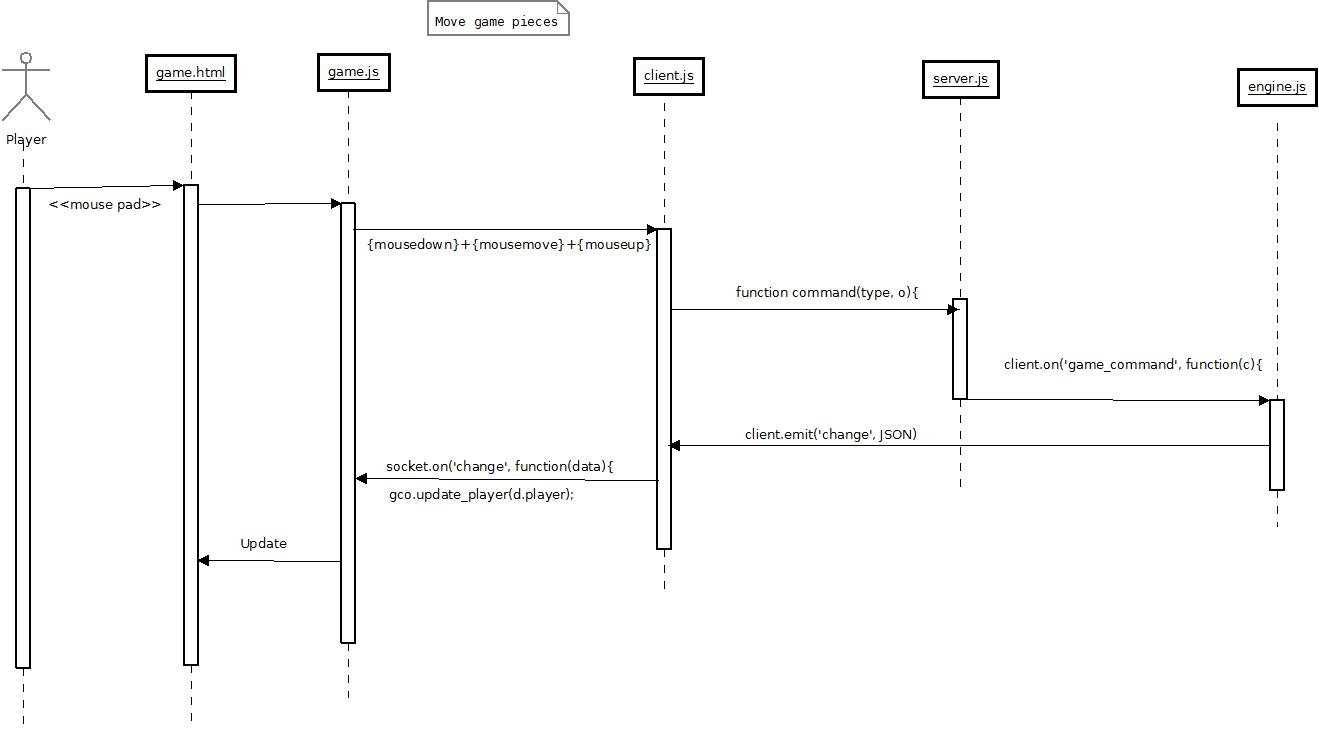
\includegraphics[width=1.0\textwidth]{img/movegamepiececsekvensdiagram.jpeg}
  \caption{Sequence diagram, 'Move game piecec'} 
  \label{fig:movegamepieceseq}
\end{figure}

The above diagram show the interaction between the JavaScript  files when a player decides to move his or hers game piece. The player initializes the sequence by clicking on the game piece in his HTML view. The first file after the HTML view is the game.js, the file that handles and interprets player inputs. The game.js file interacts with client.js which is the file handling every visual update of the game board. The file server.js Imports http and makes a server that socket.io can listen to; it connects the game interactions and game view with the engine. The file engine.js handles the game logic and game rules. When the interaction is at this point the engine.js fires a change to the client that in turn updates the view in the HTML file.\\


\begin{figure}[H]
  \centering
    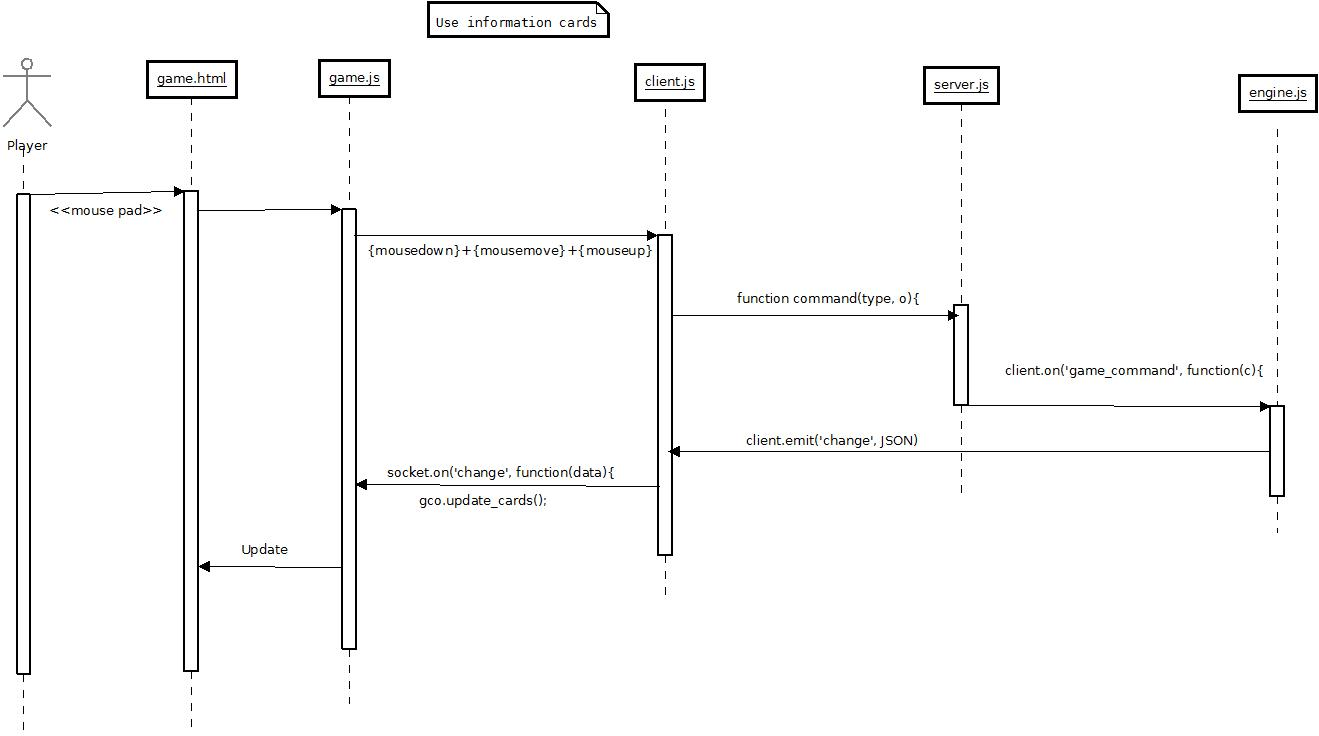
\includegraphics[width=1.0\textwidth]{img/useinfocardssekvens.jpeg}
  \caption{Sequence diagram, 'Use information card'} 
  \label{fig:useinfoseq}
\end{figure}

The above diagram shows the interactions of the JavaScript files when a player uses an information card in the game. The sequence is very similar to the previous diagram but is different in the types of data or methods it sends between the files. At the end it updates different parts of the game (gco.update();).\\


\begin{figure}[H]
  \centering
    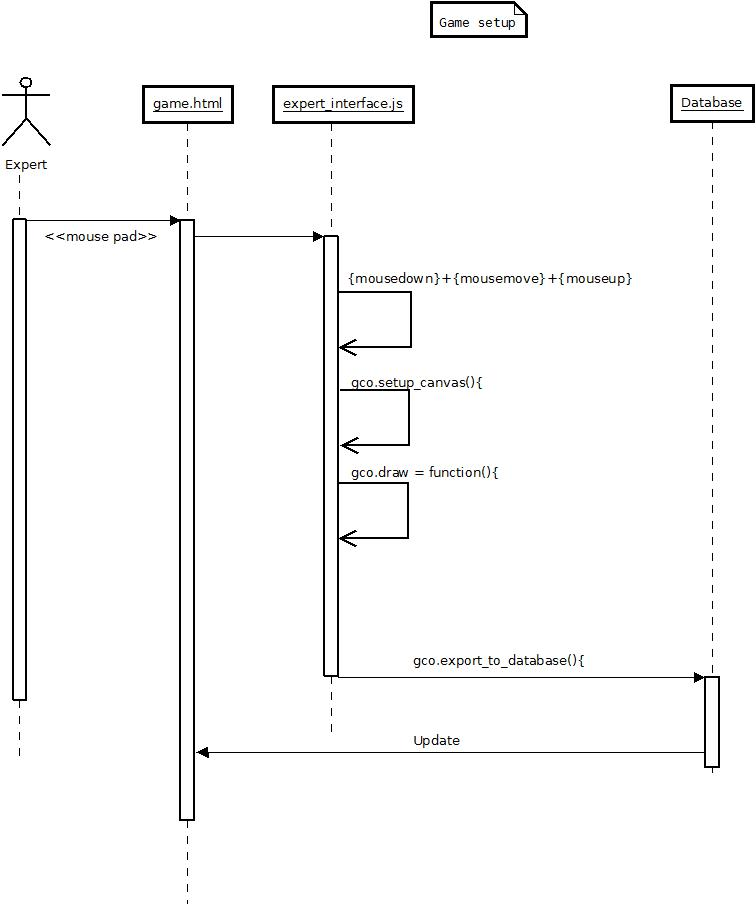
\includegraphics[width=1.0\textwidth]{img/gamesetupsekvens.jpeg}
  \caption{Sequence diagram, 'Game setup'} 
  \label{fig:gamesetupseq}
\end{figure}

The above diagram shows the interaction of the JavaScript files when an expert creates a game, the details of this is explained thoroughly in the use cases. The expert uses the mouse pad to interact with the game.html page, and is directed to the expert interface. The file expert interface.js is where all the dragging of the nodes, and creating and placing of the zones and players are created. When the expert is finished the game object is stored to the database. The last interactions is when game.html is updated when it get notifications from the database. The game can now be chosen from a list in game.html and played. 

